\chapter{Methodology}\label{chap:metodologia}
This chapter describes the tools used and the tests performed for this work. The uplink transmission of a massive MIMO system with decentralized processing (Section~\ref{subsec:uplink}) was simulated to analyze the effect of the approximation used in the inversion module of the BCD-MMSE algorithm. Based on this analysis, the fixed-point formats for the inversion module, implemented on an FPGA, are selected. The chapter begins by presenting the simulation workflow (Section~\ref{sec:simulador}) and the hardware tools (Section~\ref{sec:setup-hardware}). It then covers test configurations and conditions (Section~\ref{sec:configuracoes}), timing constraints for the inversion process (Section~\ref{sec:requisitos-tempo}), the selection of the numerical format (Section~\ref{sec:formato}), the hardware architectures, the matrices used to test them and the power estimation (Section~\ref{sec:testes-hardware}), and the organization of the results (Section~\ref{sec:organizacao-resultados}).



% =====================================================================
\section{\texorpdfstring{Simulation workflow}{Simulation workflow}}\label{sec:simulador}
% =====================================================================
The simulation workflow~\ref{fig:fluxo_simulacao} employs three tools: the QuaDRiGa channel generator, a Python simulator developed in this work, and C++ code developed in Vitis HLS, which computes the inverse of $\mathbf{G}_c$ using fixed-point arithmetic. QuaDRiGa generates the channel matrices $\mathbf{H}$ for the target UEs and $\overline{\mathbf{H}}$ for the interfering UEs.

The Python simulator handles the transmission process. It generates symbols for the target UEs and creates colored noise, with a covariance derived from $\overline{\mathbf{H}}$ (Section~\ref{subsec:ruido-colorido}), to construct the received signal using $\mathbf{H}$. Subsequently, it computes the equalizers, performs symbol detection, and measures the SER at various SNR levels. The BCD-MMSE algorithm is simulated in two ways: using the inverse of $\mathbf{G}_c$ in 64-bit floating-point format (which serves as a reference) and using the inverse in fixed-point format. In the latter case, whenever the BCD-MMSE algorithm requires $\mathbf{G}_c^{-1}$, the Python simulator invokes the C++ code.

The Python simulator models the same uplink as in \cite{zhao2025jsac}. According to the authors, that paper was the first work on decentralized processing to consider colored noise \cite{zhao2025jsac}. Therefore, the simulation parameters follow that work, except where the text indicates otherwise.



% Fluxo conferido no código:
%   QuaDRiGa: software/simulador/quadriga/export_quadriga_channels.m (semente: linha 83)
%   laço e equalizadores: dbp_sim/m1_driver.py:149-211; dbp_sim/m7_equalizers.py
%     (lmmse, zero_forcing, bdac_mmse, bcd_mmse_path); Ledoit-Wolf: dbp_sim/m5_noise.py:162-168
%   inversa em ponto fixo: dbp_sim/hls_inverse.py (usada nos resultados de SER,
%     varredura_formatos.py, bcd_inverse="hls") e dbp_sim/hw_inverse.py (modelo em Python)
% Conteúdo vem de constraints/diagramas/fluxo_simulador.puml; estrutura em caixas do
% rascunho constraints/diagramas/metodologia.svg.
\begin{figure}[!ht]
\caption{Simulation flow: QuaDRiGa channels, Python simulator and fixed-point inverse.}
\label{fig:fluxo_simulacao}
\vspace{4pt} % a classe zera o espaço entre a caption e a figura
\centering
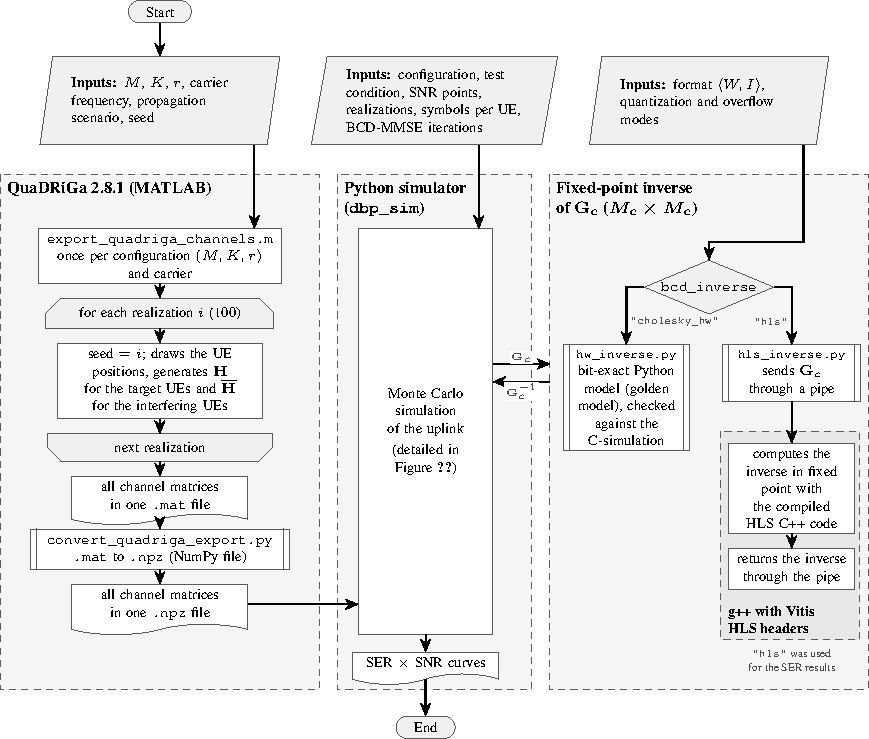
\includegraphics{Images/FLUXO/simulacao_a.pdf}
\vspace{4pt}
\legend{Source: the author.}
\end{figure}

% ---------------------------------------------------------------------
\subsection{\texorpdfstring{Channel generation}{Channel generation}}\label{subsec:simul-canal}
% ---------------------------------------------------------------------
The channels are generated using QuaDRiGa 2.8.1 in MATLAB. They depend on the number of antennas $M$, the number of target UEs $K$, the number of interfering UEs $r$, and the carrier frequency. Consequently, they are generated once for each combination of these values. Other parameters, such as $C$, the modulation scheme, and the IoTh, only affect the processing steps within the Python-based simulator. The simulation employs 100 channel realizations. Each realization consists of a random selection of UE positions, along with the corresponding channels $\mathbf{H}$ and $\overline{\mathbf{H}}$ generated by QuaDRiGa for those specific positions. Every realization uses its own unique random seed.


MATLAB saves the channels for all 100 realizations into a \texttt{.mat} file. A Python script then converts this file into an \texttt{.npz} file, NumPy’s format for storing multiple arrays within a single compressed file. The Python-based simulator reads the matrices $\mathbf{H}$ and $\overline{\mathbf{H}}$ from this file.
% ---------------------------------------------------------------------
\subsection{\texorpdfstring{Python simulator}{Python simulator}}\label{subsubsec:simul-python}
% ---------------------------------------------------------------------
The Python simulator runs two nested loops (Figure~\ref{fig:fluxo_python}). The outer loop iterates through the 100 realizations, while the inner loop iterates through the SNR points. The SNR points range from $-10$ to $10$~dB, with a step of $2$~dB. For each realization, the simulator takes $\mathbf{H}$ and $\overline{\mathbf{H}}$ corresponding to that realization and uses these channels across all SNR points. Each point on the SER curves represents the average over the 100 realizations. This is a Monte Carlo simulation, as in \cite{zhuang2025}: the SER (Section~\ref{subsubsec:ser}) is estimated by the fraction of erroneous symbols across many random draws of the channel, noise, and symbols.

At each SNR point, the simulator constructs the noise covariance matrix based on $\overline{\mathbf{H}}$, the IoTh (interference-over-thermal), and the SNR. It then generates $N$ noise samples, $\mathbf{n}^i$ (Section~\ref{subsubsec:estimacao-R}). It also generates 480 data symbols for each UE, along with the noise associated with these symbols. Based on this, the equalizers are calculated. The channel remains constant within the coherence block (Section~\ref{subsec:bloco-coerencia}); therefore, each equalizer is computed once and applied to all 480 symbols. The BCD-MMSE is compared against two centralized equalizers, the LMMSE and the ZF, which serve as benchmarks. The ZF does not utilize the noise samples $\mathbf{n}^i$. In contrast, both the LMMSE and the BCD-MMSE employ these samples to estimate the noise covariance (Section~\ref{subsubsec:condicionamento-R}). This estimate is always subjected to Ledoit-Wolf shrinkage (Equation~\ref{eq:ledoit-wolf}) before being used, even in cases where the estimate is already invertible.

In the LMMSE, this adjustment is applied to the estimate $\hat{\mathbf{R}}$ corresponding to all $M$ antennas. In the BCD-MMSE, each DU performs the adjustment on its own block, $\hat{\mathbf{R}}_{cc}$, using only the samples from its $M_c$ antennas. Consequently, no DU requires access to the samples from any other DU. The adjusted block forms the matrix $\mathbf{G}_c$ (Section~\ref{subsec:bcd}). In the reference version of the BCD-MMSE, this matrix is inverted using 64-bit floating-point arithmetic; alternatively, it can be inverted using fixed-point arithmetic (Section~\ref{subsubsec:simul-inversa}).



\begin{figure}[!ht]
\caption{Detailed flow of the Python simulator: Monte Carlo loop, equalizers and SER.}
\label{fig:fluxo_python}
\vspace{4pt} % a classe zera o espaço entre a caption e a figura
\centering
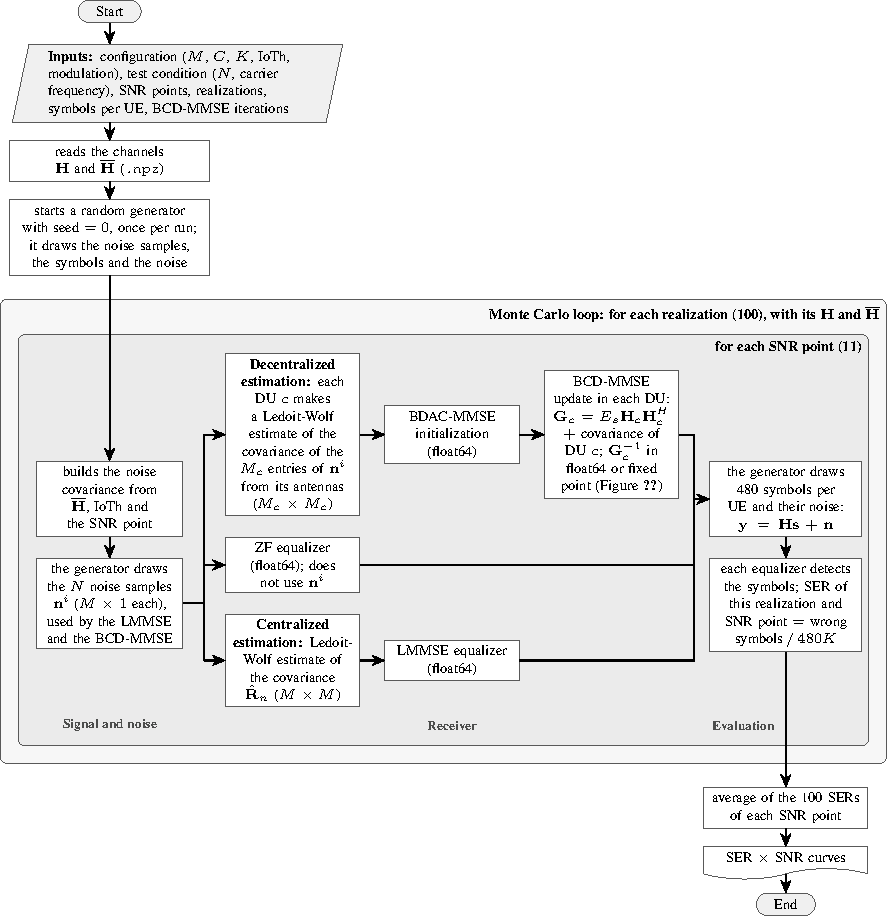
\includegraphics{Images/FLUXO/simulacao_b.pdf}
\vspace{4pt}
\legend{Source: the author.}
\end{figure}

% ---------------------------------------------------------------------
\subsection{\texorpdfstring{Fixed-point inverse}{Fixed-point inverse}}\label{subsubsec:simul-inversa}
% ---------------------------------------------------------------------
The inverse of $\mathbf{G}_c$ in fixed-point arithmetic is derived from the C++ code of the inversion module (Section~\ref{subsec:hw-modulo}). This code is compiled using \texttt{g++} along with the \texttt{ap\_fixed} header files from Vitis HLS 2026.1, with a separate compilation performed for each combination of format $\langle W, I\rangle$, quantization mode, overflow mode (Table~\ref{tab:modos-apfixed}), and size $M_c$. The program remains active throughout the simulation. Other calculations within the simulator, including the inverses used for BDAC initialization and LMMSE, utilize 64-bit floating-point arithmetic.

To verify this program, the same $\mathbf{G}_c$ matrices used in the simulator were inverted both by this program and by the Vitis HLS C-simulation. This process involved 30 matrices for each of the 35 mode combinations, with $M_c$ set to 16 and 32. In every instance, the resulting inverses were bit-identical. Consequently, the Symbol Error Rate (SER) is measured using the exact same inverse as that calculated by the hardware. The simulator also includes a Python-based model of the inversion, which has been verified bit-for-bit against the C++ code; however, the reported SER results are based on the C++ implementation.

% REMOVIDO (2026-11-05): subseção "Flow diagram". A Figura fig:fluxo_simulacao foi para a
%   abertura da seção; a frase da subseção ficou redundante com a abertura.



% =====================================================================
\section{\texorpdfstring{Hardware setup}{Hardware setup}}\label{sec:setup-hardware}
% =====================================================================
% =====================================================================
% SETUP DE HARDWARE (Metodologia) -- rascunho de 2026-11-04
% Ainda não incluído no METODOLOGIA.tex. Para incluir:
%   \section{Hardware Setup}\label{sec:setup-hardware}
%   % =====================================================================
% SETUP DE HARDWARE (Metodologia) -- rascunho de 2026-11-04
% Ainda não incluído no METODOLOGIA.tex. Para incluir:
%   \section{Hardware Setup}\label{sec:setup-hardware}
%   % =====================================================================
% SETUP DE HARDWARE (Metodologia) -- rascunho de 2026-11-04
% Ainda não incluído no METODOLOGIA.tex. Para incluir:
%   \section{Hardware Setup}\label{sec:setup-hardware}
%   \input{chapters/METODOLOGIA/setup-hardware.tex}
% Fontes do projeto (conferidas em 2026-11-04):
%   hardware/pacote_servidor_formatos/{LEIAME.md, vivado.tcl, potencia.py, rodar.sh}
%   hardware/pacote_servidor_2023/LEIAME.md
%   hardware/testes/{AMOSTRAGEM.md, LEIAME.md}
%   hardware/cholesky_hardware/{hls_config_sintese_24_12*.cfg, tb_potencia.cpp}
%   hardware/cholesky_hardware_diretivas*/LEIAME.md; acompanhamento_experimentos.csv
% Nomes das configurações: mapa LETRAS de software/testes/mapa_cenarios_v4.py
%   (antigos 1-8 = 1A,1E,1B,1F,1C,1G,1D,1H; 9-12 = 2A,2E,2B,2F).
% =====================================================================

% ---------------------------------------------------------------------
\subsection{\texorpdfstring{Tools and target device}{Tools and target device}}\label{subsec:hw-ferramentas}
% ---------------------------------------------------------------------
The inversion module was described in C++ and synthesized in Vitis HLS 2026.1. Vitis HLS generates the module's RTL. Then, the RTL was synthesized, placed, and routed in Vivado 2023.2. The target device is the AMD Alveo U50 board, with the XCU50-FSVH2104-2-E FPGA. This FPGA has 5,952 DSP blocks and 871,680 LUTs. All circuits use a clock frequency of 100 MHz, or a period of 10 ns.

In Vivado, the inversion module is synthesized and implemented alone, as the top-level design, without any other surrounding board logic. The flow performs synthesis, optimization, placement, physical optimization, and routing. The only timing constraint is the clock period, and the paths entering and exiting the module's ports are not constrained. Thus, the resource, timing, and power figures for this work are only for the module and come from the routed design in Vivado 2023.2.

Before the Vivado workflow, each version went through the Vitis HLS C synthesis. A version only went to Vivado if the HLS estimate fit within the FPGA: a maximum of 5,952 DSP blocks and a maximum of 90\% of the LUTs.

% ---------------------------------------------------------------------
\subsection{\texorpdfstring{Inversion module}{Inversion module}}\label{subsec:hw-modulo}
% ---------------------------------------------------------------------
The module receives the $M_c \times M_c$ matrix $\mathbf{G}_c$ and returns its inverse. It calculates the inverse using Cholesky decomposition (Section~\ref{sec:inversao}). Two sizes for $\mathbf{G}_c$, corresponding to the configurations described in Section~\ref{subsec:configuracoes-bs}, have been implemented: $16 \times 16$ and $32 \times 32$. The input, output, and internal values use the \texttt{ap\_fixed} data type, following the formats selected in Section~\ref{sec:formato}.

The module consists of six stages, each implemented as a C++ function (Figure~\ref{fig:modulo-inversao}). These stages are executed sequentially, with each stage passing its output to the next.
\begin{figure}[!ht]
\caption{Steps of the inversion module. Each block is one C++ function of the HLS code.}
\label{fig:modulo-inversao}
\vspace{4pt} % a classe zera o espaço entre a caption e a figura
\centering
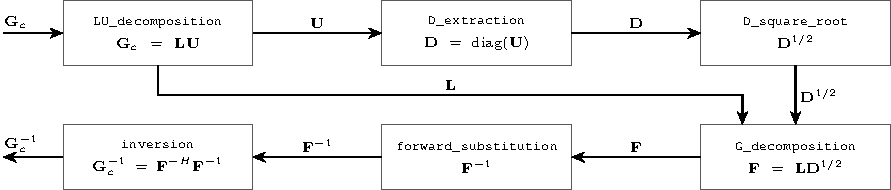
\includegraphics{Images/FLUXO/modulo_inversao.pdf}
\vspace{4pt}
\legend{Source: the author.}
\end{figure}

Additions, multiplications, and divisions utilize \texttt{ap\_fixed} type operators. Complex multiplication and division operations are explicitly implemented in the code, with a specific type defined for each intermediate value; thus, the bit-width of every intermediate value is explicitly set within the code. The addition of two $N$-bit numbers requires $N+1$ bits, while their product requires $2N$ bits \cite[pp.~72--73]{kastner-hls}. When using \texttt{ap\_fixed} types, the result of an operation inherently possesses a sufficient number of bits; overflow only occurs when this result is assigned to a type with a smaller bit-width \cite[p.~74]{kastner-hls}. Consequently, intermediate values employ types with greater bit-widths than the $\langle W, I\rangle$ format (Table~\ref{tab:tipos-intermediarios}), with the result reverting to the specified format only at the output of each stage. Square root calculations are performed using the \texttt{hls::sqrt} function from Vitis HLS, operating directly within the defined format.

\begin{table}[!ht]
\caption{Types of the values in the inversion module, for the format $\langle W, I\rangle$ with $F = W - I$ fractional bits.}
\label{tab:tipos-intermediarios}
\vspace{4pt} % a classe zera o espaço entre a caption e a tabela
\centering
\footnotesize
\renewcommand{\arraystretch}{1.2}
\begin{tabular}{p{7.4cm}cc}
\toprule
\textbf{Value} & \textbf{Integer bits} & \textbf{Fractional bits} \\
\midrule
Input, output and output of each step & $I$ & $F$ \\
Square root (\texttt{hls::sqrt}) & $I$ & $F$ \\
Accumulated sums, numerator and divisor of the complex division, quotient & $2I$ & $2F$ \\
Product of two real numbers & $4I$ & $4F$ \\
Real or imaginary part of a complex product (sum of two products) & $4I + 1$ & $4F$ \\
\bottomrule
\end{tabular}
\vspace{4pt}
\legend{Source: the author. The intermediate values use the same quantization and overflow modes as the format; the square root uses AP\_TRN and AP\_WRAP.}
\end{table}


% ---------------------------------------------------------------------

% Fontes do projeto (conferidas em 2026-11-04):
%   hardware/pacote_servidor_formatos/{LEIAME.md, vivado.tcl, potencia.py, rodar.sh}
%   hardware/pacote_servidor_2023/LEIAME.md
%   hardware/testes/{AMOSTRAGEM.md, LEIAME.md}
%   hardware/cholesky_hardware/{hls_config_sintese_24_12*.cfg, tb_potencia.cpp}
%   hardware/cholesky_hardware_diretivas*/LEIAME.md; acompanhamento_experimentos.csv
% Nomes das configurações: mapa LETRAS de software/testes/mapa_cenarios_v4.py
%   (antigos 1-8 = 1A,1E,1B,1F,1C,1G,1D,1H; 9-12 = 2A,2E,2B,2F).
% =====================================================================

% ---------------------------------------------------------------------
\subsection{\texorpdfstring{Tools and target device}{Tools and target device}}\label{subsec:hw-ferramentas}
% ---------------------------------------------------------------------
The inversion module was described in C++ and synthesized in Vitis HLS 2026.1. Vitis HLS generates the module's RTL. Then, the RTL was synthesized, placed, and routed in Vivado 2023.2. The target device is the AMD Alveo U50 board, with the XCU50-FSVH2104-2-E FPGA. This FPGA has 5,952 DSP blocks and 871,680 LUTs. All circuits use a clock frequency of 100 MHz, or a period of 10 ns.

In Vivado, the inversion module is synthesized and implemented alone, as the top-level design, without any other surrounding board logic. The flow performs synthesis, optimization, placement, physical optimization, and routing. The only timing constraint is the clock period, and the paths entering and exiting the module's ports are not constrained. Thus, the resource, timing, and power figures for this work are only for the module and come from the routed design in Vivado 2023.2.

Before the Vivado workflow, each version went through the Vitis HLS C synthesis. A version only went to Vivado if the HLS estimate fit within the FPGA: a maximum of 5,952 DSP blocks and a maximum of 90\% of the LUTs.

% ---------------------------------------------------------------------
\subsection{\texorpdfstring{Inversion module}{Inversion module}}\label{subsec:hw-modulo}
% ---------------------------------------------------------------------
The module receives the $M_c \times M_c$ matrix $\mathbf{G}_c$ and returns its inverse. It calculates the inverse using Cholesky decomposition (Section~\ref{sec:inversao}). Two sizes for $\mathbf{G}_c$, corresponding to the configurations described in Section~\ref{subsec:configuracoes-bs}, have been implemented: $16 \times 16$ and $32 \times 32$. The input, output, and internal values use the \texttt{ap\_fixed} data type, following the formats selected in Section~\ref{sec:formato}.

The module consists of six stages, each implemented as a C++ function (Figure~\ref{fig:modulo-inversao}). These stages are executed sequentially, with each stage passing its output to the next.
\begin{figure}[!ht]
\caption{Steps of the inversion module. Each block is one C++ function of the HLS code.}
\label{fig:modulo-inversao}
\vspace{4pt} % a classe zera o espaço entre a caption e a figura
\centering
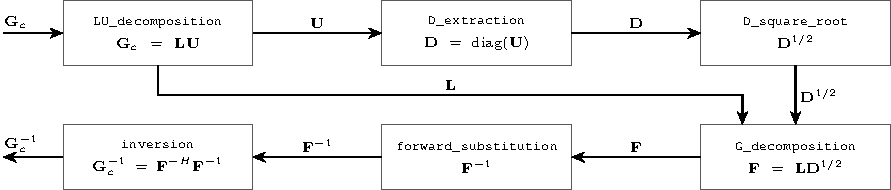
\includegraphics{Images/FLUXO/modulo_inversao.pdf}
\vspace{4pt}
\legend{Source: the author.}
\end{figure}

Additions, multiplications, and divisions utilize \texttt{ap\_fixed} type operators. Complex multiplication and division operations are explicitly implemented in the code, with a specific type defined for each intermediate value; thus, the bit-width of every intermediate value is explicitly set within the code. The addition of two $N$-bit numbers requires $N+1$ bits, while their product requires $2N$ bits \cite[pp.~72--73]{kastner-hls}. When using \texttt{ap\_fixed} types, the result of an operation inherently possesses a sufficient number of bits; overflow only occurs when this result is assigned to a type with a smaller bit-width \cite[p.~74]{kastner-hls}. Consequently, intermediate values employ types with greater bit-widths than the $\langle W, I\rangle$ format (Table~\ref{tab:tipos-intermediarios}), with the result reverting to the specified format only at the output of each stage. Square root calculations are performed using the \texttt{hls::sqrt} function from Vitis HLS, operating directly within the defined format.

\begin{table}[!ht]
\caption{Types of the values in the inversion module, for the format $\langle W, I\rangle$ with $F = W - I$ fractional bits.}
\label{tab:tipos-intermediarios}
\vspace{4pt} % a classe zera o espaço entre a caption e a tabela
\centering
\footnotesize
\renewcommand{\arraystretch}{1.2}
\begin{tabular}{p{7.4cm}cc}
\toprule
\textbf{Value} & \textbf{Integer bits} & \textbf{Fractional bits} \\
\midrule
Input, output and output of each step & $I$ & $F$ \\
Square root (\texttt{hls::sqrt}) & $I$ & $F$ \\
Accumulated sums, numerator and divisor of the complex division, quotient & $2I$ & $2F$ \\
Product of two real numbers & $4I$ & $4F$ \\
Real or imaginary part of a complex product (sum of two products) & $4I + 1$ & $4F$ \\
\bottomrule
\end{tabular}
\vspace{4pt}
\legend{Source: the author. The intermediate values use the same quantization and overflow modes as the format; the square root uses AP\_TRN and AP\_WRAP.}
\end{table}


% ---------------------------------------------------------------------

% Fontes do projeto (conferidas em 2026-11-04):
%   hardware/pacote_servidor_formatos/{LEIAME.md, vivado.tcl, potencia.py, rodar.sh}
%   hardware/pacote_servidor_2023/LEIAME.md
%   hardware/testes/{AMOSTRAGEM.md, LEIAME.md}
%   hardware/cholesky_hardware/{hls_config_sintese_24_12*.cfg, tb_potencia.cpp}
%   hardware/cholesky_hardware_diretivas*/LEIAME.md; acompanhamento_experimentos.csv
% Nomes das configurações: mapa LETRAS de software/testes/mapa_cenarios_v4.py
%   (antigos 1-8 = 1A,1E,1B,1F,1C,1G,1D,1H; 9-12 = 2A,2E,2B,2F).
% =====================================================================

% ---------------------------------------------------------------------
\subsection{\texorpdfstring{Tools and target device}{Tools and target device}}\label{subsec:hw-ferramentas}
% ---------------------------------------------------------------------
The inversion module was described in C++ and synthesized in Vitis HLS 2026.1. Vitis HLS generates the module's RTL. Then, the RTL was synthesized, placed, and routed in Vivado 2023.2. The target device is the AMD Alveo U50 board, with the XCU50-FSVH2104-2-E FPGA. This FPGA has 5,952 DSP blocks and 871,680 LUTs. All circuits use a clock frequency of 100 MHz, or a period of 10 ns.

In Vivado, the inversion module is synthesized and implemented alone, as the top-level design, without any other surrounding board logic. The flow performs synthesis, optimization, placement, physical optimization, and routing. The only timing constraint is the clock period, and the paths entering and exiting the module's ports are not constrained. Thus, the resource, timing, and power figures for this work are only for the module and come from the routed design in Vivado 2023.2.

Before the Vivado workflow, each version went through the Vitis HLS C synthesis. A version only went to Vivado if the HLS estimate fit within the FPGA: a maximum of 5,952 DSP blocks and a maximum of 90\% of the LUTs.

% ---------------------------------------------------------------------
\subsection{\texorpdfstring{Inversion module}{Inversion module}}\label{subsec:hw-modulo}
% ---------------------------------------------------------------------
The module receives the $M_c \times M_c$ matrix $\mathbf{G}_c$ and returns its inverse. It calculates the inverse using Cholesky decomposition (Section~\ref{sec:inversao}). Two sizes for $\mathbf{G}_c$, corresponding to the configurations described in Section~\ref{subsec:configuracoes-bs}, have been implemented: $16 \times 16$ and $32 \times 32$. The input, output, and internal values use the \texttt{ap\_fixed} data type, following the formats selected in Section~\ref{sec:formato}.

The module consists of six stages, each implemented as a C++ function (Figure~\ref{fig:modulo-inversao}). These stages are executed sequentially, with each stage passing its output to the next.
\begin{figure}[!ht]
\caption{Steps of the inversion module. Each block is one C++ function of the HLS code.}
\label{fig:modulo-inversao}
\vspace{4pt} % a classe zera o espaço entre a caption e a figura
\centering
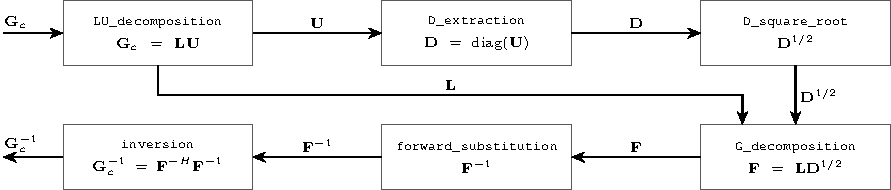
\includegraphics{Images/FLUXO/modulo_inversao.pdf}
\vspace{4pt}
\legend{Source: the author.}
\end{figure}

Additions, multiplications, and divisions utilize \texttt{ap\_fixed} type operators. Complex multiplication and division operations are explicitly implemented in the code, with a specific type defined for each intermediate value; thus, the bit-width of every intermediate value is explicitly set within the code. The addition of two $N$-bit numbers requires $N+1$ bits, while their product requires $2N$ bits \cite[pp.~72--73]{kastner-hls}. When using \texttt{ap\_fixed} types, the result of an operation inherently possesses a sufficient number of bits; overflow only occurs when this result is assigned to a type with a smaller bit-width \cite[p.~74]{kastner-hls}. Consequently, intermediate values employ types with greater bit-widths than the $\langle W, I\rangle$ format (Table~\ref{tab:tipos-intermediarios}), with the result reverting to the specified format only at the output of each stage. Square root calculations are performed using the \texttt{hls::sqrt} function from Vitis HLS, operating directly within the defined format.

\begin{table}[!ht]
\caption{Types of the values in the inversion module, for the format $\langle W, I\rangle$ with $F = W - I$ fractional bits.}
\label{tab:tipos-intermediarios}
\vspace{4pt} % a classe zera o espaço entre a caption e a tabela
\centering
\footnotesize
\renewcommand{\arraystretch}{1.2}
\begin{tabular}{p{7.4cm}cc}
\toprule
\textbf{Value} & \textbf{Integer bits} & \textbf{Fractional bits} \\
\midrule
Input, output and output of each step & $I$ & $F$ \\
Square root (\texttt{hls::sqrt}) & $I$ & $F$ \\
Accumulated sums, numerator and divisor of the complex division, quotient & $2I$ & $2F$ \\
Product of two real numbers & $4I$ & $4F$ \\
Real or imaginary part of a complex product (sum of two products) & $4I + 1$ & $4F$ \\
\bottomrule
\end{tabular}
\vspace{4pt}
\legend{Source: the author. The intermediate values use the same quantization and overflow modes as the format; the square root uses AP\_TRN and AP\_WRAP.}
\end{table}


% ---------------------------------------------------------------------


% =====================================================================
\section{\texorpdfstring{Configurations and test conditions}{Configurations and test conditions}}\label{sec:configuracoes}
% =====================================================================
\subsection{\texorpdfstring{Base station configurations}{Base station configurations}}\label{subsec:configuracoes-bs}
The uplink of the massive MIMO system was investigated using two types of parameters. Hard constraints refer to the physical characteristics of the base station: $M = 128$ or 256 antennas, $C = 8$ or 16 clusters, and the size $M_c = M/C$ of the inversion module. Soft constraints depend on the UEs being served and the level of interference: $K = 8$ or 12 UEs, QPSK or 16-QAM modulation, and an IoTh ratio of 10 dB as a baseline case, or 20 dB representing an extreme, high-interference scenario. These configurations were adapted from \cite{zhao2025jsac}. Table~\ref{tab:paineis} presents these configurations.


Each configuration is identified by a label consisting of a number and a letter. The number denotes the hard constraints: 1 for $M = 128$ and $C = 8$; 2 for $M = 256$ and $C = 8$; and 3 for $M = 256$ and $C = 16$. The letter indicates the soft constraints and remains consistent across all three groups.

\begin{table}[htbp]
\caption{Simulated configurations.}
\label{tab:paineis}
\vspace{4pt} % a classe zera o espaço entre a caption e a tabela
\centering
\footnotesize
\renewcommand{\arraystretch}{1.2}
% sem espaço em volta das linhas do booktabs, para as bordas verticais não terem falhas
\setlength{\aboverulesep}{0pt}
\setlength{\belowrulesep}{0pt}
\begin{tabular}{|c|c|c|c|c|c|c|}
\toprule
\multirow{2}{*}{\textbf{Configuration}} & \multicolumn{3}{c|}{\textbf{Hard constraints}} & \multicolumn{3}{c|}{\textbf{Soft constraints}} \\
\cline{2-7}
 & {\boldmath $M$} & {\boldmath $C$} & {\boldmath $M_c$} & \textbf{IoTh (dB)} & \textbf{Modulation} & {\boldmath $K$} \\
-- & \texttt{M} & \texttt{C} & -- & \texttt{iot\_db} & \texttt{modulation} & \texttt{K} \\
\midrule
1A & \multirow{8}{*}{128} & \multirow{8}{*}{8} & \multirow{8}{*}{16} & \multirow{4}{*}{10} & \multirow{2}{*}{16-QAM} & 8 \\
1B & & & & & & 12 \\
\cline{6-7}
1C & & & & & \multirow{2}{*}{QPSK} & 8 \\
1D & & & & & & 12 \\
\cline{5-7}
1E & & & & \multirow{4}{*}{20} & \multirow{2}{*}{16-QAM} & 8 \\
1F & & & & & & 12 \\
\cline{6-7}
1G & & & & & \multirow{2}{*}{QPSK} & 8 \\
1H & & & & & & 12 \\
\midrule
2A & \multirow{8}{*}{256} & \multirow{8}{*}{8} & \multirow{8}{*}{32} & \multirow{4}{*}{10} & \multirow{2}{*}{16-QAM} & 8 \\
2B & & & & & & 12 \\
\cline{6-7}
2C & & & & & \multirow{2}{*}{QPSK} & 8 \\
2D & & & & & & 12 \\
\cline{5-7}
2E & & & & \multirow{4}{*}{20} & \multirow{2}{*}{16-QAM} & 8 \\
2F & & & & & & 12 \\
\cline{6-7}
2G & & & & & \multirow{2}{*}{QPSK} & 8 \\
2H & & & & & & 12 \\
\midrule
3A & \multirow{8}{*}{256} & \multirow{8}{*}{16} & \multirow{8}{*}{16} & \multirow{4}{*}{10} & \multirow{2}{*}{16-QAM} & 8 \\
3B & & & & & & 12 \\
\cline{6-7}
3C & & & & & \multirow{2}{*}{QPSK} & 8 \\
3D & & & & & & 12 \\
\cline{5-7}
3E & & & & \multirow{4}{*}{20} & \multirow{2}{*}{16-QAM} & 8 \\
3F & & & & & & 12 \\
\cline{6-7}
3G & & & & & \multirow{2}{*}{QPSK} & 8 \\
3H & & & & & & 12 \\
\bottomrule
\end{tabular}

\vspace{4pt}
\legend{Source: 1A, 1B, 1C, 1E, 2A and 3A adapted from \citesp{zhao2025jsac}; the others, the author. $r = 8$ in all configurations. Second header row: field names of \texttt{Panel} in the code.}

\end{table}

% AUTORA (9-results.tex:245) -- parágrafo retirado do texto (tom); o conteúdo ficou em comentário.
% Configurações 1, 9, 13, 3, 2, 5 = painéis (a), (b), (c), (e), (f), (g) da Fig. 8 de Zhao et al.
% O painel (d) não aparece no artigo. Na configuração 3 (painel e), r = 8 foi
% mantido; L577 liga r a K, então r = 12 também seria defensável.




\subsection{Test conditions}\label{subsec:setup_condicoes}
% Criado em 2026-11-04 (reorganização pedida pela autora): junta o que define as condições
%   de teste. Origens: RESULTADOS/setup_simulacao.tex (subsubseção "Test Conditions", texto da
%   autora, e Tabela tab:condicoes_teste); METODOLOGIA/simulacao.tex (parágrafo do N);
%   METODOLOGIA/formato.tex (TDLA30-5 e TDLA30-10 com as mesmas curvas).

The simulated test conditions of Table~\ref{tab:n-maximo} define the carrier frequency and the number of noise samples in the Python simulator, as shown in Table~\ref{tab:condicoes_teste}. The simulation does not include a time axis, and the channel does not account for the Doppler effect, so only these two variables change between test conditions. A frequency of 3.5 GHz was used for FR1 conditions, within the n78 band (3300 to 3800 MHz, TDD), and 28 GHz was used for FR2 conditions, within the n257 band (26500 to 29500 MHz, TDD) \cite[Tabs.~5.2-1 and 5.2-2]{3gpp-ts38104}. In each realization, the channels at both frequencies use the same UE positions. % TODO: 3,5 GHz não tem fonte. Sugestão: citar uma referência que use 3,5 GHz como banda típica do 5G NR (ex.: livro 5G and Beyond), ou dizer só que é uma escolha deste trabalho.


\begin{table}[htbp]
\caption{Carrier frequency and number of noise samples in each test condition.}
\label{tab:condicoes_teste}
\vspace{4pt} % a classe zera o espaço entre a caption e a tabela
\centering
\footnotesize
\renewcommand{\arraystretch}{1.2}
\begin{tabular}{ccccc}
\toprule
\textbf{Test condition} & \textbf{\shortstack{Frequency\\range}} & \textbf{\shortstack{Carrier\\frequency (GHz)}} & \textbf{\shortstack{Noise\\samples {\boldmath $N$}}} & \textcolor{red}{\textbf{\shortstack{UE speed\\(km/h)}}} \\
\texttt{M1\_Driver.} & -- & \texttt{M1\_Driver.} & \texttt{M5\_Noise.} & -- \\
\texttt{test\_conditions} & & \texttt{test\_conditions} & \texttt{n\_noise\_samples} & \\
\midrule
TDLA30-5 & FR1 & 3.5 & 192 & \textcolor{red}{1.5} \\
TDLA30-10 & FR1 & 3.5 & 192 & \textcolor{red}{3.1} \\
TDLA30-75 & FR2 & 28 & 192 & \textcolor{red}{2.9} \\
TDLA30-300 & FR2 & 28 & 168 & \textcolor{red}{11.6} \\
TDLC300-100 & FR1 & 3.5 & 132 & \textcolor{red}{30.8} \\
TDLB100-400 & FR1 & 3.5 & 24 & \textcolor{red}{123.3} \\
\bottomrule
\end{tabular}

\vspace{4pt}
% FONTE (velocidade): v = f_D c / f_c, Tse e Viswanath p. 70; f_D de TS 38.104 Tab. G.2.2-1/G.2.2-2; antes na Tabela tab:tempo-coerencia (retirada).
\legend{Source: \citesp{3gpp-ts38104} and the author. \textcolor{red}{Speed from $v = f_D c/f_c$ \citesp{tse-viswanath}.}}
\end{table}

This work employs a double-symbol DM-RS, located at symbols 2, 3, 10, and 11 of each slot \cite[Tab.~6.4.1.1.3-4]{3gpp-ts38211}, as it enables the differentiation of DM-RS signals among $K = 8$ or 12 UEs (Section~\ref{subsubsec:disponibilidade-amostras}). The value of $N$ for each condition is taken from Table~\ref{tab:n-maximo}, with an upper limit of 192, the value used in \cite{zhao2025jsac}. This $N$ assumes that the receiver waits for samples arriving after the data symbol (Section~\ref{subsec:pipeline}). The HST350 and HST500 conditions were not simulated, as they correspond to $N = 0$.

TDLA30-5 and TDLA30-10 share the same carrier frequency and the same $N$ value. Consequently, they exhibit identical SER curves, and the simulations cover 5 distinct test conditions. The only difference between them lies in the inversion cycle limit (Section~\ref{subsec:restricao-vazao}).

The test conditions are grouped into two mobility profiles based on UE speed (Table~\ref{tab:condicoes_teste}). The low-mobility profile includes TDLA30-5, TDLA30-10, and TDLA30-75, with speeds up to 3.1 km/h. The high-mobility profile comprises TDLA30-300, TDLC300-100, and TDLB100-400, with speeds ranging from 11.6 to 123.3 km/h. The ITU-R uses 3 km/h for indoor and pedestrian users, and 30 and 120 km/h for users in vehicles \cite[Sec.~8.2 and Tab.~5]{itu-m2412}. In each profile, the fastest condition is the most demanding: it has the smallest $T_c$ and the smallest $N$. This condition is TDLA30-75 in the low-mobility profile and TDLB100-400 in the high-mobility profile.

% FONTE ITU: Rep. ITU-R M.2412-0, Sec. 8.2 (p. 16): Indoor Hotspot "stationary and pedestrian",
%   Dense Urban "pedestrian and vehicular", Rural "pedestrian, vehicular and high speed vehicular";
%   Tab. 5a (p. 20): indoor 3 km/h; Tab. 5b (p. 23): indoor 3 km/h, in-car 30 km/h;
%   Tab. 5c (p. 25): indoor 3 km/h, 120 km/h e 500 km/h. Arquivo: books/R-REP-M.2412-2017-PDF-E.pdf.


% =====================================================================
\section{\texorpdfstring{Inversion cycle limit}{Inversion cycle limit}}\label{sec:requisitos-tempo}
% =====================================================================
This section calculates, based on the coherence time, the maximum number of cycles between two inversions under each test condition.

% ---------------------------------------------------------------------
\subsection{\texorpdfstring{Sample collection}{Sample collection}}\label{subsec:pipeline}
% ---------------------------------------------------------------------
The receiver first collects the $N$ noise samples for each PRB. Some of these samples arrive only after the data symbol (Section~\ref{subsubsec:disponibilidade-amostras}). Therefore, this work assumes that the receiver buffers the data symbols until the $N$ samples have been received. Subsequently, it processes the samples and equalizes the buffered data. A new set of samples arrives every interval $T_c$, and the processing must keep pace with this rate.

% ---------------------------------------------------------------------
\subsection{Throughput}\label{subsec:restricao-vazao}
% ---------------------------------------------------------------------
The estimate $\hat{\mathbf R}_{cc}$ is unique per PRB within each interval $T_c$ (Section~\ref{subsubsec:disponibilidade-amostras}). The matrix $\mathbf G_c$ is inverted once and serves all iterations of the BCD-MMSE algorithm (Section~\ref{subsec:bcd}). Thus, each DU performs one inversion of $\mathbf G_c$ per PRB every $T_c$. With $N_{\text{PRB}}$ PRBs, this results in $N_{\text{PRB}}$ inversions per DU every $T_c$. This work uses $N_{\text{PRB}} = 275$, which is the worst-case scenario for 5G NR (Section~\ref{subsec:simbolos}).

To track data collection, the module needs to complete the $N_{\text{PRB}}$ inversions within $T_c$. Let $T_{\text{inv}}$ be the interval between the start of two inversions (Section~\ref{subsubsec:latencia-intervalo}). Then:
\begin{equation}
{T_{\text{inv}} \leq \frac{T_c}{N_{\text{PRB}}}.}
\label{eq:restriction-flow}
\end{equation}
With a clock speed of 100 MHz (Section~\ref{subsec:hw-ferramentas}), this limit is given in cycles, rounded down. Table~\ref{tab:limite-ciclos} shows the limit for each test condition.

\begin{table}[!ht]
\caption{Maximum interval between inversions in each test condition.}
\label{tab:limite-ciclos}
\vspace{4pt} % a classe zera o espaço entre a caption e a tabela
\centering
\footnotesize
\renewcommand{\arraystretch}{1.2}
\begin{tabular}{lccc}
\toprule
\textbf{Test condition} & {\boldmath $T_c$} \textbf{(ms)} & {\boldmath $T_c/N_{\text{PRB}}$} \textbf{(\textmu s)} & \textbf{Limit at 100 MHz (cycles)} \\
\midrule
TDLA30-5    & 25.0000 & 90.9091 & 9090 \\
TDLA30-10   & 12.5000 & 45.4545 & 4545 \\
TDLA30-75   & 1.6667  & 6.0606  & 606 \\
TDLA30-300  & 0.4167  & 1.5152  & 151 \\
TDLC300-100 & 1.2500  & 4.5455  & 454 \\
TDLB100-400 & 0.3125  & 1.1364  & 113 \\
\bottomrule
\end{tabular}
\vspace{4pt}
\legend{Source: the author. $T_c$ from Table~\ref{tab:n-maximo}; $N_{\text{PRB}} = 275$.}
\end{table}

The hardware architectures in this work aim to meet this throughput limit under each test condition. The following are outside the scope: the delay between the arrival of a data symbol and its equalization; the throughput of the links between the DUs; and the other matrix inversions required by the BCD-MMSE algorithm, which the simulator performs using floating-point arithmetic (Section~\ref{subsubsec:simul-inversa}). The delay encompasses both the time spent waiting for samples and the latency of each inversion (i.e., the time elapsed from the start to the completion of an inversion).


% =====================================================================
\section{\texorpdfstring{Selection of the fixed-point format}{Selection of the fixed-point format}}\label{sec:formato}
% =====================================================================
% ---------------------------------------------------------------------
% 1.5  ESCOLHA DO FORMATO DE PONTO FIXO          -> nova seção da Metodologia
% ---------------------------------------------------------------------
% ORIGEM: TCC/Análise bits.md (resumo da autora), com as correções de 2026-11-04:
%   nomes 1A-3D no lugar das letras A-P; IoTh; "condição de teste" no lugar de
%   "cenário"; critério de escolha lexicográfico (não a razão perda/ocupação);
%   5 formatos finais (não 3); AP_TRN_ZERO corrigido; tabela de velocidades
%   retirada (já está em FUNDAMENTACAO/modelo-de-canal.tex).

\subsection{\texorpdfstring{SNR increase}{SNR increase}}\label{subsec:aumento-snr}

To select the $\langle W, I\rangle$ format (Section~\ref{subsubsec:ponto-fixo}), the BCD-MMSE algorithm was simulated using both fixed-point and 64-bit floating-point matrix inversion. Only the inversion of $\mathbf G_c$ differs between the two simulations; however, the SNR and SER are measured for the entire uplink. Each format was evaluated based on the SNR increase, that is, the additional SNR required by the uplink to achieve an $\mathrm{SER} = 10^{-2}$ compared to the floating-point case. This increase corresponds to the horizontal distance between the two SER curves, which is the standard method for comparing two schemes \cite[p.~55]{tse-viswanath}.

% grade de SNR: params.M1_Driver.snr_db_grid (-10 a 10, passo 2); QPSK a partir de -20 dB:
%   curvas_qpsk_256 (grupos 2 e 3) e curvas_qpsk_128 (grupo 1), referencia_qpsk_256.py
\textcolor{red}{As curvas de SER foram simuladas de $-10$ a 10~dB, com passo de 2~dB. Com QPSK, a grade começa em $-20$~dB, porque algumas curvas já atingem $\mathrm{SER} = 10^{-2}$ antes de $-10$~dB: quase todas as do LMMSE no grupo 1 e todas as do LMMSE e do BCD-MMSE nos grupos 2 e 3.}

Two thresholds were employed. A 0.1~dB threshold represents a near-ideal format, where the SER curve is virtually identical to that of the floating-point implementation. A 3~dB threshold serves as the maximum acceptable increase. An increase of 3~dB is equivalent to doubling the power \cite[p.~73]{tse-viswanath}. Consequently, at this threshold, each UE would need to transmit with twice the energy per symbol to compensate for the error introduced by the matrix inversion (Section~\ref{subsec:snr}).



\subsection{\texorpdfstring{Initial sweep}{Initial sweep}}
The first stage involved varying the integer and fractional parts separately, while keeping the other part fixed (Table~\ref{tab:varredura-inicial}). Each size was tested across 35 combinations of quantization and overflow modes (Table~\ref{tab:modos-apfixed}), using the BCD-MMSE algorithm with both 1 and 4 iterations.

\begin{table}[htbp]
\caption{Sizes tested in the initial sweep.}
\label{tab:varredura-inicial}
\vspace{4pt} % a classe zera o espaço entre a caption e a tabela
\centering
\footnotesize
\renewcommand{\arraystretch}{1.2}
\begin{tabular}{lll}
\toprule
\textbf{Sweep} & \textbf{Integer bits} ({\boldmath $I$}) & \textbf{Fractional bits} ({\boldmath $F$}) \\
\midrule
Integer part & 6, 8, 10, 12, 14, 16, 20, 24, 32 & 32 \\
Fractional part & 14 & 4, 6, 8, 10, 12, 16, 20, 24, 32 \\
\bottomrule
\end{tabular}
\vspace{4pt}
\legend{Source: the author.}
\end{table}
% NOTA: 9 + 9 = 18 tamanhos, mas <46,14> (I = 14, F = 32) aparece nas duas
%   varreduras: 17 tamanhos por varredura de configuração e condição.

\subsection{\texorpdfstring{Configurations of the initial sweep}{Configurations of the initial sweep}}
The initial sweep utilized the 16 configurations for which the floating-point SER curve reaches $10^{-2}$ within the $-10$ to $10$ dB range. Running all of these across the 5 test conditions would have resulted in 80 cases, each involving 17 sizes and 35 mode combinations; therefore, only 5 configurations were selected.


The selection process relied on the $\mathbf{G}_c$ matrices at two SNR points surrounding the operating point (defined as $\mathrm{SER} = 10^{-2}$ in floating-point arithmetic). From each matrix, the largest absolute value between the real and imaginary parts of the elements was taken, since the circuit stores the two parts separately. This value is referred to here as the ``maximum $|$part$|$''. In each case, the 99th percentile of these values was used to ensure that the overall ranking would not be disproportionately influenced by a few outlier matrices. Larger elements necessitate a greater number of integer bits. Configurations 1G, 1H, 2E, and 2F contain the largest elements and are the most demanding, while configuration 1A contains the smallest elements and was used as a baseline (Table~\ref{tab:gc-ponto-operacao}).


These configurations also span the extremes of precision requirements. With a limited number of bits, the rounding error in matrix inversion increases with the condition number \cite[p.~1603]{osinsky2023}. When the smallest eigenvalue is very small, the matrix approaches a singular state, making the result more dependent on the fractional part (Section~\ref{subsubsec:ponto-fixo}). Configurations 2E and 2F exhibit the highest condition numbers (at the 99th percentile), whereas configuration 1A features the smallest eigenvalues (at the 1st percentile).


\begin{table}[htbp]
\caption{$\mathbf{G}_c$ at the operating point of the initial-sweep configurations.}
\label{tab:gc-ponto-operacao}
\vspace{4pt} % a classe zera o espaço entre a caption e a tabela
\centering
\footnotesize
\renewcommand{\arraystretch}{1.2}
\setlength{\tabcolsep}{4pt}
\begin{tabular}{ccccccccc}
\toprule
 & \multicolumn{2}{c}{\textbf{SNR (dB)}} & \multicolumn{2}{c}{\textbf{Largest} {\boldmath $|$}\textbf{part}{\boldmath $|$}} & \multicolumn{2}{c}{\textbf{Condition number}} & \multicolumn{2}{c}{\textbf{Smallest eigenvalue}} \\
\cmidrule(lr){2-3}\cmidrule(lr){4-5}\cmidrule(lr){6-7}\cmidrule(lr){8-9}
\textbf{Configuration} & \textbf{192; 3.5} & \textbf{168; 28} & \textbf{192; 3.5} & \textbf{168; 28} & \textbf{192; 3.5} & \textbf{168; 28} & \textbf{192; 3.5} & \textbf{168; 28} \\
\midrule
1A & $-2.6$ & $-2.4$ & 63   & 66   & 57  & 58  & 1.9  & 1.9 \\
1G & $-9.3$ & $-9.1$ & 2266 & 2383 & 187 & 169 & 22.4 & 24.1 \\
1H & $-8.7$ & $-8.6$ & 2470 & 2385 & 195 & 172 & 22.1 & 24.7 \\
2E & $-5.8$ & $-5.6$ & 962  & 999  & 286 & 254 & 8.8  & 9.7 \\
2F & $-5.6$ & $-5.5$ & 983  & 987  & 282 & 285 & 8.8  & 9.5 \\
\bottomrule
\end{tabular}
\vspace{4pt}
\legend{Source: the author. Subcolumns: $N$; carrier in GHz.}

\end{table}

\subsection{\texorpdfstring{Synthesis and selection of formats for validation}{Synthesis and selection of formats for validation}}

The sizes and modes of the initial sweep were also synthesized in Vitis HLS to measure resource occupancy (LUT, DSP, FF, and BRAM). The occupancy of each circuit is that of the most used resource in the FPGA. In each configuration and test condition, the integer and fractional parts with the lowest occupancy were chosen, with an SNR increase of up to 3 dB and of up to 0.1 dB, in 1 and in 4 iterations. Combining the two parts resulted in 10 formats (Table~\ref{tab:formatos-origem}).


\begin{table}[htbp]
\caption{Configurations in which each format was chosen in the initial sweep.}
\label{tab:formatos-origem}
\vspace{4pt} % a classe zera o espaço entre a caption e a tabela
\centering
\footnotesize
\renewcommand{\arraystretch}{1.2}
\begin{tabular}{ccccc}
\toprule
 & \multicolumn{2}{c}{\textbf{1 iteration}} & \multicolumn{2}{c}{\textbf{4 iterations}} \\
\cmidrule(lr){2-3}\cmidrule(lr){4-5}
\textbf{Format} & \textbf{Up to 3~dB} & \textbf{Up to 0.1~dB} & \textbf{Up to 3~dB} & \textbf{Up to 0.1~dB} \\
\midrule
$\langle 14,6\rangle$  & 1A         & --                       & --             & --                       \\
$\langle 16,6\rangle$  & --         & --                       & 1A             & --                       \\
$\langle 18,8\rangle$  & --         & 1A                       & --             & --                       \\
$\langle 20,8\rangle$  & --         & --                       & --             & 1A                       \\
$\langle 22,12\rangle$ & 1H, 2E, 2F & --                       & --             & --                       \\
$\langle 24,12\rangle$ & 1G         & 2E, 2F                   & 1G, 1H, 2E, 2F & --                       \\
$\langle 26,12\rangle$ & --         & 1G$^{a}$, 1H$^{a}$       & --             & 2E, 2F                   \\
$\langle 28,12\rangle$ & --         & --                       & --             & 1G$^{a}$, 1H$^{a}$       \\
$\langle 28,14\rangle$ & --         & 1G$^{b}$, 1H$^{b}$       & --             & --                       \\
$\langle 30,14\rangle$ & --         & --                       & --             & 1G$^{b}$, 1H$^{b}$       \\
\bottomrule
\end{tabular}
\vspace{4pt}
\legend{Source: the author. Columns: SNR increase. No mark: all 5 test conditions. $^{a}$Only TDLB100-400. $^{b}$The other 4 conditions.}
\end{table}



\subsection{\texorpdfstring{Validation}{Validation}}\label{subsec:validacao}
The initial sweep fixed one part of the word while varying the other, and used only 5 configurations. This can change the most used resource and the best mode. Therefore, the 10 formats were simulated again, with the 35 mode combinations, in the 24 configurations and 5 test conditions.

In this step, BCD-MMSE used only 1 iteration. The 4 iterations of the initial sweep had already helped to choose the formats of the most demanding cases: $\langle 16,6\rangle$, $\langle 20,8\rangle$, $\langle 28,12\rangle$ and $\langle 30,14\rangle$ only appeared with 4 iterations (Table~\ref{tab:formatos-origem}). With 1 iteration, BCD-MMSE already has a good result in SER. Furthermore, the inverse of $\mathbf G_c$ is calculated once and used in all iterations, so the number of inversions does not change (Section~\ref{subsec:bcd}).

The circuit has only one mode. Therefore, each format received a fixed mode in each group of configurations (Section~\ref{sec:configuracoes}). All configurations in a group use the same circuit. The mode was chosen according to the following criteria, in this order:

\begin{enumerate}

\item the mode that leaves more pairs (configuration, test condition) with an increase in SNR of up to 3~dB. A pair that does not reach $\mathrm{SER} = 10^{-2}$ counts as out of bounds;
\item the lowest resource occupancy, by the most used resource in the synthesis;
\item  the quantization \texttt{AP\_RND\_ZERO}, which never uses more resources than the other tied modes;

\item the smallest increase in SNR in the worst pair;
\item the order of the modes in the list.

\end{enumerate}

% FONTE: grade curta = varredura_formatos.grade_perto (--snr-perto, extra_direita 2), [4] v4 e
%   v5; grade inteira = rodadas [5] (modo_fixo_3dB, _iot10, _qpsk_128, _qpsk_256) e
%   rodada6_mapa_grade_inteira.sh (modo_fixo_mapa, 2026-11-08), semente 0 como a referência.
\textcolor{red}{Nessa etapa, a simulação em ponto fixo usou só as SNRs em volta do ponto de operação, com passo de 2~dB. Elas começam no ponto da grade logo abaixo da SNR em que o BCD-MMSE em ponto flutuante atinge $\mathrm{SER} = 10^{-2}$ e vão de 4 a 7~dB além dela. Depois de escolhido o modo fixo, cada formato foi simulado de novo, só com esse modo, na grade inteira de SNR (Seção~\ref{subsec:aumento-snr}). Essas simulações usam a mesma semente da simulação em ponto flutuante. A escolha dos três formatos de cada grupo e os resultados da Seção~\ref{sec:resultados-formato} vêm delas.}

% ANTIGO: Then, with the fixed mode, three formats were chosen in each group. The first is the smallest format in which all configurations and conditions of the group reach $\mathrm{SER} = 10^{-2}$, with any increase in SNR. The second and third are the smallest, where all reach this point with an increase of up to 3 dB and up to 0.1 dB, respectively. These formats were implemented in Vivado and are in the Section \ref{sec:resultados-formato}.
\textcolor{red}{Depois, com o modo fixo, foram escolhidos dois formatos em cada grupo: o menor em que todas as configurações e condições do grupo atingem $\mathrm{SER} = 10^{-2}$ com aumento de SNR de até 3~dB, e o menor com aumento de até 0,1~dB. O aumento é arredondado em duas casas decimais. O menor formato que só atinge $\mathrm{SER} = 10^{-2}$, com qualquer aumento, não foi usado como critério, porque esse aumento chega a mais de 10~dB (Seção~\ref{sec:resultados-formato}). Esses formatos foram implementados no Vivado e estão na Seção~\ref{sec:resultados-formato}.}

% =====================================================================
\section{\texorpdfstring{Hardware architectures, test matrices and power}{Hardware architectures, test matrices and power}}\label{sec:testes-hardware}
% =====================================================================
% Separado de setup-hardware.tex em 2026-11-04: as ferramentas e o módulo ficam antes
%   (ferramentas); as arquiteturas, as matrizes de teste e a potência vêm depois do formato.
The chosen formats were synthesized using Vitis HLS. In all versions, the automatic loop pipelining feature was disabled \cite[p.~42]{ug1399}. The first version, without loop optimizations, was implemented for both $16 \times 16$ and $32 \times 32$ matrix sizes. In this version, the iterations of each loop execute sequentially, and the $N_{\text{PRB}} = 275$ matrices within a block are inverted one by one. Consequently, the interval between inversions exceeds the limits defined for all test conditions (Table~\ref{tab:limite-ciclos}), and the module does not track the arrival of the matrices at each $T_c$.

To meet the cycle limits for each test condition, a specific architecture was developed for every case, only in $16 \times 16$, with Vitis HLS directives that reduce the interval between inversions. All versions were implemented in Vivado, tested using $\mathbf G_c$ matrices obtained from the simulator (Section~\ref{subsec:hw-matrizes}), and evaluated for power consumption and energy per inversion (Section~\ref{subsec:hw-potencia}). Each version produces the same inverse as the non-optimized implementation, a result verified bit-for-bit against the C-language code.
% FONTE: hardware/viabilidade_32x32/LEIAME.md (síntese C, HLS 2026.1 local, 2026-11-02, <24,12>).
\textcolor{red}{As arquiteturas otimizadas não foram implementadas em $32 \times 32$. Uma síntese C de teste das seis, em $32 \times 32$ e no formato $\langle 24,12\rangle$, estimou intervalos acima do limite de ciclos de todas as condições de teste. Nas sistólicas, o intervalo cresce 4 vezes, com o quadrado do tamanho da matriz. A da TDLB100-400 também não caberia no FPGA. Para atender os limites em $32 \times 32$, seria preciso outra arquitetura, com mais área, e isso não foi testado.}

\subsection{\texorpdfstring{Hardware architectures}{Hardware architectures}}\label{subsec:hw-arquiteturas}
% ---------------------------------------------------------------------
All optimized architectures employ pipelining (Section~\ref{subsubsec:latencia-intervalo}). Every $T_c$, the DU inverts 275 matrices $\mathbf G_c$, one for each PRB (Section~\ref{sec:requisitos-tempo}). For the 9,090 and 4,545-cycle limits, the module inverts one matrix at a time. For tighter limits, it inverts the matrices in batches of $n$. In all cases, the module must receive the 275 matrices for a given block within the duration $T_c$.

The matrices within a batch are independent of one another. Consequently, $c$ of these matrices are computed in the same cycle using loop unrolling, which creates a copy of the loop body for each iteration. The loop that iterates over the $c$ matrices is nested within a pipelined loop, and the HLS tool performs the unrolling automatically \cite[pp.~41, 372, and 428]{ug1399}. When $c$ is less than $n$, groups of $c$ matrices are processed in alternating cycles. Each copy has its own dedicated memory bank, though it may share operators with the others.

The values for $n$ and $c$ were determined through trial and error and are presented in Table~\ref{tab:hw-arquiteturas}.
 

\begin{table}[htbp]
\caption{Batch of the inversion module in each test condition.}
\label{tab:hw-arquiteturas}
\vspace{4pt} % a classe zera o espaço entre a caption e a tabela
\centering
\footnotesize

\renewcommand{\arraystretch}{1.2}
\setlength{\tabcolsep}{4pt}
\begin{tabular}{lcccc}
\toprule
\textbf{Test condition} & \begin{tabular}[c]{@{}c@{}}\textbf{Limit per}\\\textbf{matrix (cycles)}\end{tabular} & \begin{tabular}[c]{@{}c@{}}\textbf{Matrices per}\\\textbf{batch} ({\boldmath $n$})\end{tabular} & \begin{tabular}[c]{@{}c@{}}\textbf{Copies}\\({\boldmath $c$})\end{tabular} & \begin{tabular}[c]{@{}c@{}}\textbf{Batches}\\\textbf{per block}\end{tabular} \\
\midrule
Without optimizations & --    & 1  & 1 & 275 \\
TDLA30-5    & 9090 & 1  & 1 & 275 \\
TDLA30-10   & 4545 & 1  & 1 & 275 \\
TDLA30-75   & 606   & 12 & 6 & 23 \\
TDLC300-100 & 454   & 16 & 8 & 18 \\
TDLA30-300  & 151   & 32 & 2 & 9 \\
TDLB100-400 & 113   & 32 & 4 & 9 \\
\bottomrule
\end{tabular}

\vspace{4pt}
\legend{Source: the author. Limit per matrix from Table~\ref{tab:limite-ciclos}.}
\end{table}



% ---------------------------------------------------------------------
\subsubsection{\texorpdfstring{Loop pipelining}{Loop pipelining}}\label{subsubsec:hw-pipeline-lacos}

The module consists of six sequential stages (Figure~\ref{fig:modulo-inversao}): LU decomposition, extraction of the diagonal $\mathbf D$, calculation of the square root $\mathbf D^{1/2}$, computation of $\mathbf F$, forward substitution, and inversion. For the 9,090-cycle limit, the internal loops of these stages are annotated with the \texttt{\#pragma HLS pipeline II=1} directive. The \texttt{D\_extraction} stage is the only one without this directive, as it merely copies the diagonal from $\mathbf U$ to $\mathbf D$ and requires significantly fewer cycles than the other stages.

This directive enables loop pipelining, specifying that a new iteration should begin every cycle, that is, an initiation interval (II) of 1 cycle (Section~\ref{subsubsec:latencia-intervalo}). If data dependencies or resource constraints prevent this, the HLS tool will automatically use a larger II \cite[p.~45]{kastner-hls}.

Figure~\ref{fig:hw-pipeline-lacos} illustrates a loop from the LU decomposition process, both without and with pipelining. The individual stages and loops for a given matrix are executed sequentially. Consequently, the next inversion process cannot begin until the current one has finished; in this case, the interval between inversions is equal to the latency \cite[p.~114]{kastner-hls}.

\begin{figure}[!ht]
\caption{Loop pipelining in the LU decomposition. The code is simplified.}
\label{fig:hw-pipeline-lacos}
\vspace{4pt} % a classe zera o espaço entre a caption e a figura
\centering
\begin{minipage}[c]{0.62\textwidth}
\fontsize{8}{9.6}\selectfont
\begin{verbatim}
for (line = column + 1; line < n; line++)
  for (k = column; k < n; k++) {
#pragma HLS pipeline II=1
    t = L[line][column] * U[column][k];
    U[line][k] = U[line][k] - t;
  }
\end{verbatim}
\end{minipage}

\vspace{8pt}
\begin{minipage}[c]{\textwidth}
\centering
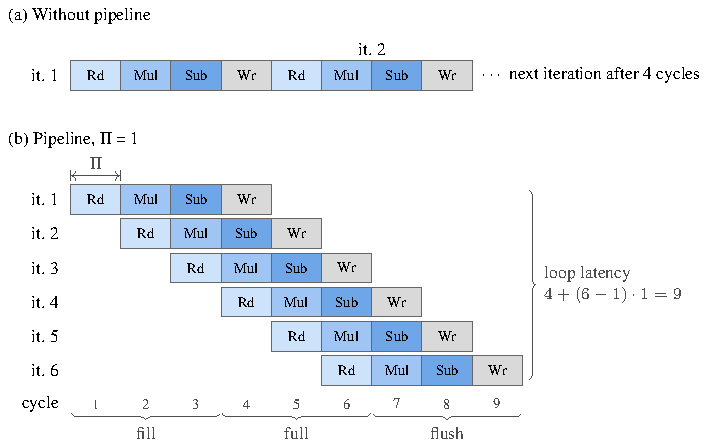
\includegraphics{Images/FLUXO/hw_pipeline_lacos.pdf}
\end{minipage}
\vspace{4pt}
\legend{Source: the author. Rd: read, Mul: multiply, Sub: subtract, Wr: write. Iteration latency of 4 cycles, for illustration.}
\end{figure}

% ---------------------------------------------------------------------
\subsubsection{\texorpdfstring{Dataflow between stages}{Dataflow between stages}}\label{subsubsec:hw-dataflow}

The architecture of the 4,545-cycle limit maintains the loop pipeline and combines the six steps into four: LU decomposition, calculation of $\mathbf F$ (\texttt{D\_extraction}, \texttt{D\_square\_root} and \texttt{G\_decomposition}), forward substitution, and inversion. The \texttt{\#pragma HLS dataflow} directive, applied to the top-level function, implements a task-level pipeline across the four stages, with each stage assigned to a specific matrix (Section~\ref{subsubsec:pipeline-tarefas}). Each step carries the directive \texttt{\#pragma HLS inline off}, which keeps it as a separate function \cite[p.~52]{kastner-hls}. In Figure~\ref{fig:hw-dataflow}, the latency of a matrix is the sum of the four steps, and the interval is the duration of the longest step.

% FONTE: cholesky_hardware_diretivas_4545/cholesky_top.cpp (etapa_lu, etapa_g, etapa_fs,
%   etapa_inv; dataflow em cholesky_inverse, linha 68). Kastner p. 52 (inline off mantém a
%   hierarquia), p. 114 (dataflow: as funções executam ao mesmo tempo, em dados diferentes).
%   Intervalo = etapa mais longa: Kastner p. 115 (na Fundamentação).

\begin{figure}[!ht]
\caption{Dataflow between the stages of the inversion. The code is simplified.}
\label{fig:hw-dataflow}
\vspace{4pt}
\centering
\begin{minipage}[c]{0.45\textwidth}
\fontsize{8}{9.6}\selectfont
\begin{verbatim}
void cholesky_inverse(A, inverse) {
#pragma HLS dataflow
  etapa_lu(A, L, U);
  etapa_g(U, L, G);
  etapa_fs(G, G_inv);
  etapa_inv(G_inv, inverse);
}

static void etapa_fs(G, G_inv) {
#pragma HLS inline off
  forward_substitution(G, G_inv);
}
\end{verbatim}
\end{minipage}

\vspace{8pt}
\begin{minipage}[c]{\textwidth}
\centering
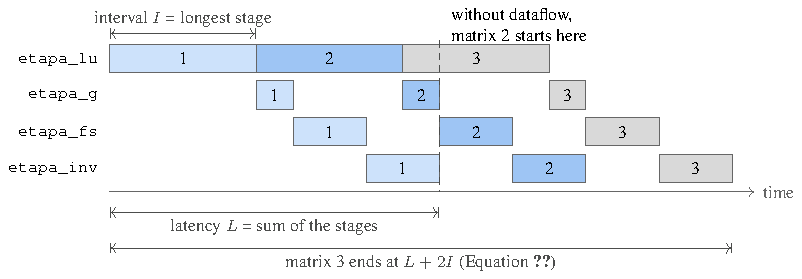
\includegraphics{Images/FLUXO/hw_c2.pdf}
\end{minipage}
\vspace{4pt}
\legend{Source: the author. Numbers in the boxes: index of the matrix.}
\end{figure}

% ---------------------------------------------------------------------
\subsubsection{\texorpdfstring{Matrix batches}{Matrix batches}}\label{subsubsec:hw-lotes}


Within the 606 and 454 cycle limits, the steps form a dataflow, as in the 4,545 cycle limit. The $c$ copies read different matrices in the same cycle, but a BRAM memory only allows access to two addresses per cycle. Therefore, the batch memory is divided into $c$ BRAM banks, one per copy, using the directive \texttt{\#pragma HLS array\_partition cyclic} and factor $c$. Thus, matrix $m$ is located in bank $m \bmod c$ \cite[pp.~87--88]{kastner-hls}.

Figure~\ref{fig:hw-lotes} shows the architecture of the 606 cycle limit. Since the two groups of 6 matrices alternate in each cycle, one iteration does not wait for the result of the previous one. Each copy has its own multipliers, but there is a single divider in each step, shared by the copies. It receives one matrix of the batch per cycle and, since it has a pipeline, it also does not wait for the previous division.

\begin{figure}[!ht]
\caption{Batch of 12 matrices with 6 copies, for the 606-cycle limit. The code is simplified.}
\label{fig:hw-lotes}
\vspace{4pt}
\centering
\begin{minipage}[c]{0.62\textwidth}
\fontsize{8}{9.6}\selectfont
\begin{verbatim}
#pragma HLS array_partition variable=U \
                     cyclic factor=COPIES dim=1
for (k = column; k < n; k++)
  for (g = 0; g < GRUPOS; g++) {
#pragma HLS pipeline II=1
    for (p = 0; p < COPIES; p++) {
      m = g * COPIES + p;
      t = L[m][line][column] * U[m][column][k];
      U[m][line][k] = U[m][line][k] - t;
    }
  }
\end{verbatim}
\end{minipage}

\vspace{8pt}
\begin{minipage}[c]{\textwidth}
\centering
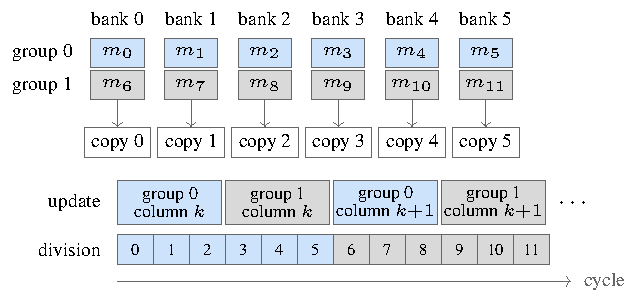
\includegraphics{Images/FLUXO/hw_c3.pdf}
\end{minipage}
\vspace{4pt}
\legend{Source: the author. Bank $p$ holds the matrices with $m \bmod 6 = p$. Update: 6 matrices per cycle. Division: one matrix $m$ per cycle, in a single divider.}
\end{figure}

% ---------------------------------------------------------------------
\subsubsection{\texorpdfstring{Systolic arrays}{Systolic arrays}}\label{subsubsec:hw-sistolico}

Within the 151 and 113-cycle limits, the stages also form a dataflow, with each copy featuring its own divider. LU decomposition, forward substitution, and inversion utilize systolic arrays: the $k$-loop, which iterates over a row or a summation, is nested within a pipelined loop, which HLS unrolls into 16 processing elements (PEs) (Section~\ref{subsubsec:arranjo-sistolico}). Each stage employs an array structure per copy, resulting in a total of $3c$ such arrays within the module.

In forward substitution and inversion, each PE adds a term and passes the partial sum to the next PE, following the same sequence as the unoptimized version, with each cycle computing a complete sum. In the LU decomposition, each cycle updates an entire row, with one element assigned to each PE. To achieve this, each row element is stored in its own dedicated register, configured using the \texttt{\#pragma HLS array\_partition complete} directive \cite[p.~87]{kastner-hls}.

In both LU decomposition and forward substitution, each step reads rows that were written during the previous step, with a cycle offset corresponding to the step size. During the final steps of the LU decomposition and the initial steps of the forward substitution, which are relatively short, the required row might still be within the pipeline. Consequently, these steps are padded with empty cycles until they reach a minimum duration (Figure~\ref{fig:hw-sistolico}). Since HLS cannot automatically infer this from the source code, the \texttt{\#pragma HLS dependence ... dependent=false} directive is used to specify that the iterations are independent of one another \cite[p.~149]{kastner-hls}.


\begin{figure}[!ht]
\caption{Systolic array of the forward substitution and minimum step of the LU decomposition. The code is simplified.}
\label{fig:hw-sistolico}
\vspace{4pt}
\centering
\begin{minipage}[c]{0.62\textwidth}
\fontsize{8}{9.6}\selectfont
\begin{verbatim}
#pragma HLS array_partition variable=Ua \
                     complete dim=3
for (it = 0; it < LU_ITER; it++) {
#pragma HLS pipeline II=1
#pragma HLS dependence variable=Ua \
          type=inter dependent=false
  if (idx < reais)       // else: empty
    for (p = 0; p < COPIES; p++)
      for (k = 0; k < n; k++)  // PEs
        Ua[m][line][k] = row[k] - l*piv[k];
}
\end{verbatim}
\end{minipage}

\vspace{8pt}
\begin{minipage}[c]{\textwidth}
\centering
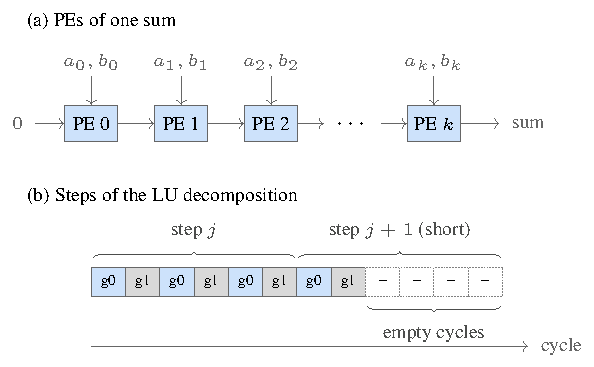
\includegraphics{Images/FLUXO/hw_c4.pdf}
\end{minipage}
\vspace{4pt}
\legend{Source: the author. g0, g1: groups of matrices of the batch, one per cycle; there are 16 groups for the 151-cycle limit and 8 for the 113-cycle limit.}
\end{figure}

% ---------------------------------------------------------------------
\subsection{\texorpdfstring{Test matrices}{Test matrices}}\label{subsec:hw-matrizes}
% ---------------------------------------------------------------------
The hardware was tested with the same $\mathbf{G}_c$ matrices that BCD-MMSE inverts in the SER curves, with 1 iteration. These matrices were saved before inversion, in each of the 5 distinct test conditions (Section~\ref{subsec:setup_condicoes}). In each condition, a sample was saved: some matrices randomly selected by configuration and SNR point, and the most extreme in range and precision, such as those with the largest element and the largest condition number. QPSK configurations were excluded because the modulation does not change $\mathbf{G}_c$.

The testbench inverts 20 matrices randomly selected from this sample. In the $16 \times 16$ circuit, these matrices come only from configurations 1A--1H. In architectures with batch, the 20 matrices are repeated until at least 3 batches are completed.


% FONTE: rodar_potencia.py (sinteses/*_vivado/potencia/): 20 matrizes sorteadas com
%   semente fixa; 16x16: 1A, 1B, 1E e 1F; 32x32: 2A, 2B, 2E e 2F; grupo 3 fora da potência
%   (decisão da autora). tb_potencia.cpp da 606 (linhas 57-71: lotes = max(3, ceil(20/LOTE)));
%   potencia.csv: 36 (606), 48 (455), 96 (152 e 114), 20 nas outras.

% ---------------------------------------------------------------------
\subsection{\texorpdfstring{Power and energy}{Power and energy}}\label{subsec:hw-potencia}
% ---------------------------------------------------------------------
Power was estimated from the switching activity of the routed design: the version without optimizations under the 5 test conditions, and each optimized architecture only under its own. Vivado generates a functional netlist, which is simulated with the testbench. The simulation checks the inverses byte by byte against the C code and records how many times each signal changes value in a SAIF (Switching Activity Interchange Format) file. Vivado then reads this file and reports the power.

Energy per inversion is defined as the dynamic power multiplied by the average time required for an inversion. This duration is calculated as the interval between two inversions, measured during the netlist simulation, multiplied by the 10~ns clock period. In architectures that employ batch processing, the interval between two batches is divided by $n$.
\textcolor{red}{A potência estática é a potência total menos a dinâmica.}
% Retirado em 2026-11-13 (a figura potencia_media_condicao saiu dos Resultados em 2026-11-09):
%   A potência média no ritmo exigido de cada condição de teste soma a potência estática e a
%   energia de 275 inversões dividida por T_c. Ela supõe que, depois de inverter as 275 matrizes
%   do bloco, o módulo fica parado até o próximo bloco e só gasta a potência estática.
% FONTE: memória tcc-pacote-servidor-2023 (convenção da energia). Intervalo tirado do
%   xsim_<cenário>.log do servidor, não do ciclos_medios do potencia.csv, que inclui o
%   enchimento do pipeline do primeiro lote.


% =====================================================================
% \section{\texorpdfstring{Organization of the results}{Organization of the % results}}\label{sec:organizacao-resultados}
% =====================================================================


% ---------------------------------------------------------------------
% 1.6  ORGANIZAÇÃO DOS RESULTADOS                 -> fim da Metodologia
% ---------------------------------------------------------------------
% The results are grouped according to the physical characteristics of the base station: the size of the inversion circuit ($16 \times 16$ or $32 \times 32$), the number of antennas $M$, and the number of clusters $C$. Within each group, the modulation, $K$, and IoTh vary. Thus, there are three groups: configurations 1A–1H ($M = 128$, $C = 8$, $16 \times 16$ circuit), 2A–2H ($M = 256$, $C = 8$, $32 \times 32$ circuit), and 3A–3H ($M = 256$, $C = 16$, $16 \times 16$ circuit). \textcolor{red}{Os mapas de aumento de SNR, as curvas, as barras e os perfis de mobilidade são apresentados por grupo (Seção~\ref{sec:resultados-formato}). Os resultados de hardware, de vazão e de atraso são apresentados por condição de teste (Seção~\ref{sec:resultados-hardware}).}

